% !TeX encoding = UTF-8

\documentclass[12pt,a4paper,openany,
               afrikaans,UKenglish,
               masters-t,goldenblock 
              ]{stb-thesis} 

%==== Language setup =================================================
\usepackage{babel}
\usepackage[utf8]{inputenc}%...................... Unicode input file format

%==== Math setup =====================================================
\usepackage{amsmath}%............................. Advanced math (before fonts)
%\usepackage{amssymb}%............................ AMS Symbol fonts

%==== Font setup (default is Computer Modern) ========================
\usepackage{iftex}
\ifxetex
    \usepackage[math-style=TeX,
                bold-style=TeX,
               ]{unicode-math}
    \setmainfont{Times New Roman}%........................ Unicode fonts  (Win)
    \setsansfont[Scale=MatchLowercase]{Calibri}
    \setmonofont[Scale=MatchLowercase]{Consolas}
    \setmathfont{Cambria Math}
    \defaultfontfeatures{Ligatures=TeX}
    \let\bm\symbfit
\else
    \usepackage[utf8]{inputenc}%.................. Unicode file format
    \usepackage{textcomp}%........................ Additional text symbols
    \usepackage[T1]{fontenc}%..................... Type 1 outline fonts
    % Use Times (newtx) as a pdfLaTeX fallback for Times New Roman
    \usepackage{newtxtext,newtxmath}
    \usepackage{bm}%.............................. Bold math fonts
\fi
\normalfont

%==== Units and numbers ==============================================
\usepackage{siunitx}%............................. Unit, number and angle output
    \sisetup{detect-all = true, detect-family = true}
    \sisetup{%output-decimal-marker = {.} ,
             group-separator = {\,},
             number-unit-product = {\,},
             inter-unit-product = \mathord{\cdot},
             exponent-product = \mathord{\times},
             separate-uncertainty = true}
   
         
%==== Ref's, Bib's and Nomencl =======================================
\usepackage{stb-nomencl}%......................... List of symbols 
    \renewcommand*{\UnitLabel}[1]{~[\,$\unit{#1}$\,]}
\usepackage{stb-bib}%............................. Bibliography (natbib internally)
    \bibliographystyle{stb-bib-eng-a}
    \renewcommand\bibfont{\small}
    \renewcommand\bibsection{\chapter{\bibname}}

%==== Tables + Graphics + Color =====================================
\usepackage{array}%............................... Extended table defs 
    \setlength{\extrarowheight}{2pt}
\usepackage{longtable}%........................... Tables can break over pages
\usepackage{graphicx}%............................ Included graphics
\usepackage[font=small]{caption}%................. Customize captions  
\usepackage[table]{xcolor}%....................... Color setup + colortbl 
    
%==== Extra defs for template ========================================
\makeatletter
%---- TOC entries and case
    \addto{\captionsafrikaans}{\renewcommand\bibname{Lys van verwysings}}
    \addto{\captionsafrikaans}{\renewcommand\contentsname{Inhoudsopgawe}}
    \addto{\captionsafrikaans}{\renewcommand\listfigurename{Lys van figure}}
    \addto{\captionsafrikaans}{\renewcommand\listtablename{Lys van tabelle}}

    \addto{\captionsUKenglish}{\renewcommand{\bibname}{List of references}}
    \addto{\captionsUKenglish}{\renewcommand\contentsname{Table of contents}}
    \addto{\captionsUKenglish}{\renewcommand\listfigurename{List of figures}}
    \addto{\captionsUKenglish}{\renewcommand\listtablename{List of tables}}

%==== User Defs ======================================================
%
% Please insert user defined commands here
% and NOT in the document itself!
\usepackage{soul}
\usepackage{parskip}
\usepackage{titlesec}
\usepackage{float}
\usepackage{graphicx}
\usepackage{subcaption}
\usepackage[hidelinks]{hyperref}
\usepackage{pgfgantt}   
\usepackage{pdflscape} 
\usepackage{longtable}
\usepackage{booktabs}
\usepackage{array} 
\usepackage{tabularx}
\usepackage{colortbl}
\usepackage[table]{xcolor}
\usepackage{ragged2e}
\usepackage{caption}
\usepackage{placeins}

\renewcommand{\@makechapterhead}[1]{%
  \vspace*{-40pt}% <-- move chapter heading up (adjust if needed)
  {\parindent \z@ \raggedright \normalfont
    \ifnum \c@secnumdepth >\m@ne
        \huge\bfseries \@chapapp\space \thechapter
        \par\nobreak
        \vskip 10pt
    \fi
    \Huge \bfseries #1\par\nobreak
    \vskip 40pt
  }}


%%==== End of user defs =================================================

\makeatother

%==== Title Page =====================================================
\title{\bfseries
       \AorE{%-- Afrikaans ------------------------------------------
             Diskrete Element Modellering van 'n Vibrerende Skeurploeg\\[1ex]
             \normalfont\small\itshape
             (``Discrete Element Modeling of a Vibratory Subsoiler'')
            }{%-- English -------------------------------------------
             User-Defined Gesture Control System for Photography Drones}}

\author{C.\ Wiid}{Caleb Wiid}

\degree{\AorE{MIng (Meg)}{MEng (Mech)}}
       {\AorE{Magister in Ingenieurswese (Meganiese)}
             {Master of Engineering (Mechanical)}}

\address{\AorE{%-- Afrikaans ----------------------------------------
        Departement Meganiese en Megatroniese Ingenieurswese,\\
        Stellenbosch Universiteit,\\
        Privaatsak X1, Matieland 7602, Suid Afrika.%
             }{%-- English ------------------------------------------
        Department of Mechanical and Mechatronic Engineering,\\
        Stellenbosch University,\\
        Private Bag X1, Matieland 7602, South Africa.}}

\faculty{\AorE{Fakulteit Ingenieurswese}%
              {Faculty of Engineering}}

\supervisor{Dr.\ W\ Smit}

\setdate{\the\month}{\the\year}

%\SetSponsor{The financial assistance of the National Research Foundation (NRF)
%    towards this research is hereby acknowledged. Opinions expressed and
%    conclusions arrived at, are those of the author and are not necessarily to
%    be attributed to the NRF.}


%==== Main Document ==================================================
\setcounter{secnumdepth}{3}
\setcounter{tocdepth}{2}
\raggedbottom
\begin{document}   

\frontmatter%---------------------------------------------------------                    
\TitlePage

\DeclarationDate{2026/05/15}
\DeclarationPage

\begin{abstract}[english]%===================================================
Drones are increasingly used in fields such as photography, inspection, and emergency response, yet their operation still requires specialist training and conventional control interfaces that can be difficult for non-experts to use. This project investigates a gesture-controlled drone system that allows users to define and personalise their own hand gestures for controlling a drone in a more natural way.

The proposed system will focus on learning user-specific gestures rather than forcing all users to adapt to a fixed gesture vocabulary. To support this, the project will explore few-shot learning methods for recognising new gestures from only a small number of examples, while retaining a small set of fixed safety-critical commands such as take-off, landing, return home, and emergency stop. The prototype will be implemented and evaluated on a physical drone to assess whether personalised gesture learning can provide reliable control for both basic flight and photography-oriented functions.

By combining gesture recognition, incremental learning, and real-world drone testing, the project aims to contribute to Human-Robot Interaction research and to demonstrate a more accessible and adaptable approach to drone control.
\end{abstract}


%\include{chaps-front/chap-acknowledge}
%\include{chaps-front/chap-dedication}

% Use \chapter*{} before TOC
\tableofcontents
% Use \chapter{} after TOC

\listoffigures
\listoftables
%\include{chaps-front/chap-symbols}

\mainmatter%----------------------------------------------------------
\numberwithin{figure}{chapter}
\numberwithin{table}{chapter}

\chapter{Introduction}

\section{Background}

Drones, or Unmanned Aerial Vehicles (UAVs), are becoming increasingly important across many industries. They show great promise in simplifying logistics, reducing costs, improving human safety, and providing faster response times and more accurate results \citep{Patrona2021}. Their effectiveness has been demonstrated across a wide variety of sectors, including agriculture, search and rescue, surveillance, transportation, and photography \citep{DronesInAction2025}. Despite these advantages, effective drone operation currently requires specialist training, limiting accessibility for many potential users \citep{International_journal_of_engineering_research_2017}.

This has created demand for systems that allow users to control drones in a more natural and intuitive way. The field of Human-Robot Interaction (HRI) focuses on the study and design of communication between humans and robots \citep{HRI_sciencedirect}, and has driven the emergence of Natural User Interfaces (NUIs). NUIs encompass a range of technologies, including touchscreens, voice recognition, eye tracking, and gesture recognition \citep{Natural_UI}. This project will focus on gesture control as a natural interface for operating a photography drone.

Gesture control enables users to communicate with digital systems through natural hand and body movements, removing the need for traditional input devices \citep{Anjua2024}. Research has shown that, without prior instruction, humans naturally attempt to communicate with drones through gestures \citep{Gio2021}, suggesting that gesture-based control aligns closely with instinctive human behaviour. This has practical implications as gesture-based drone control lowers the barrier to entry to drones by removing the need for specialist training \citep{Mehta2023}. Additionally, gesture control has been shown to enable both experienced and novice pilots to operate drones more effectively \citep{Gio2021}.

Despite these advances, current gesture-based control systems remain limited in their flexibility. Most existing approaches rely on fixed, predefined gesture vocabularies that all users must conform to, with no accommodation for individual differences in movement style or preference \citep{Reyes2023}. This lack of personalisation represents a clear gap in the research, which this project aims to address.

\section{Aim}

The aim of this project is to develop a gesture-controlled photography and videography drone that allows users to create and personalise their own gestures. Rather than conforming to a fixed set of predefined gestures, the system will learn and adapt to gestures chosen by the user, giving them full control over how they will interact with the drone.

A small set of core gestures will remain fixed for essential safety-critical functions such as take-off, landing, emergency stop, and return home. All other functions will be fully customisable, allowing the user to assign any gesture they choose to a specific task.

The drone will support a range of operations, from basic flight controls such as movement and rotation, to more complex photography-specific movements including tracking shots, dronies\footnote{A dronie is a cinematic shot where the drone moves backward and upward while keeping the subject centred in the frame}, spotlight shots, and reveal shots.

\section{Objectives}

In order to achieve this aim, the following objectives must be met:
\begin{itemize}
    \item Implement system on a physical drone. 
    \item Recognise and interpret basic gestures.
    \item Control basic drone functions using basic gestures.
    \item Learn unique user-defined gestures and assign them to photography-specific functions.
    \item Perform photography-specific functions.
    \item Manage similar or ambiguous gestures reliably.
\end{itemize}

\section{Motivation}

Gesture-based drone control presents compelling alternative to traditional contollers. By leveraging the natural human motor skills of a person, it allows users to interact with a drone in a more natural way, reducing the complexity associated with conventional control interfaces \citep{Trinitatova2025}. As a result, this will greatly improve the accessibility as users without prior piloting experience. \cite{Taylor2025} has stated that people without prior piloting experience have been shown to operate gesture-controlled drones safely and intuitively, particularly when combined with features such as obstacle avoidance and 3D trajectory mapping \citep{Taylor2025}.

Beyond accessibility, gesture control can reduce cognitive load by enabling more instantaneous and instinctive command inputs, which is particularly valuable in time-critical applications such as search and rescue or disaster relief scenarios \citep{Kumar2020}. Lightweight, real-time gesture recognition algorithms have further demonstrated that a manageable set of gestures can support precise and nuanced drone manoeuvres without overwhelming the user \citep{Yun2024}. Incorporating personalisation takes this further, allowing the intuitive nature of gesture interaction to be fully realised for each individual user.

\section{Scope}

The primary focus of this project is the gesture recognition system. Specifically, how accurately the system can recognise, classify, and learn new gestures. To achieve this, Few-Shot Learning (FSL) will be used, enabling the system to recognise a new gesture from only a small number of examples. This is essential for a system designed to learn from the user in real time.

A photography drone was chosen as the platform for testing because it offers a wide and complex range of tasks, making it an ideal testbed. Although the underlying system could be applied to many other domains; such as agriculture, search and rescue, or surveillance; the photography use case was selected as it presents the greatest variety of distinct functions. If the system performs effectively in this context, it is logical to assume that it will also be effective in other industries.

The key gaps this project addresses are:
\begin{itemize}
    \item The lack of truly personalised gesture control, where the user rather than the designer defines the gesture vocabulary.
    \item The challenge of incremental gesture learning — how a system can be introduced to a new gesture, correctly classify it, and reliably distinguish it from similar gestures going forward.
\end{itemize}
\chapter{Literature review}
This chapter will discuss the current state of the art technology that incorporates gesture recognition to control the movement of a drone as well as gesture recognition as a whole. This chapter will discuss the various forms of gesture control, the learning algorithems behind gesture recognition and categorisation, and the current implementations of gesture control for drones. 

\section{Types of Gesture Control}
\subsection{Image-Based vs Non-Image-Based Gesture Recognition}
According to \cite{Khaksar2023} there are two general approaches when it comes to gesture recognition and data acquisition: image-based and non-image-based approaches. The image-based approach can be further categorised into three main subcategories which include depth camera detection, stereo camera detection and single camera detection as shown in Figure \ref{fig:gesture_sensors} \citep{Khaksar2023}. This approach makes use of cameras to capture a gesture and then using feature extraction, transforms this information into usable data that a system can use.

The non-image based approach on the other hand makes use of sensors to capture a gesture. These sensors are catogorised into glove devices and band devices. Typically these devices make use of Inertial Measurment Units (IMUs) in combination with flex sensors to capture the movement of a hand or arm \citep{muezzinoglu2021}. This method typically more robust to environmenteal factors (such as lighting conditions) compared to image-based approachs, however the recent trend has been to move to image-based approachces as they are less intrusive and more userfriendly \citep{Gio2021}.

\begin{figure} [htbp]
    \centering
    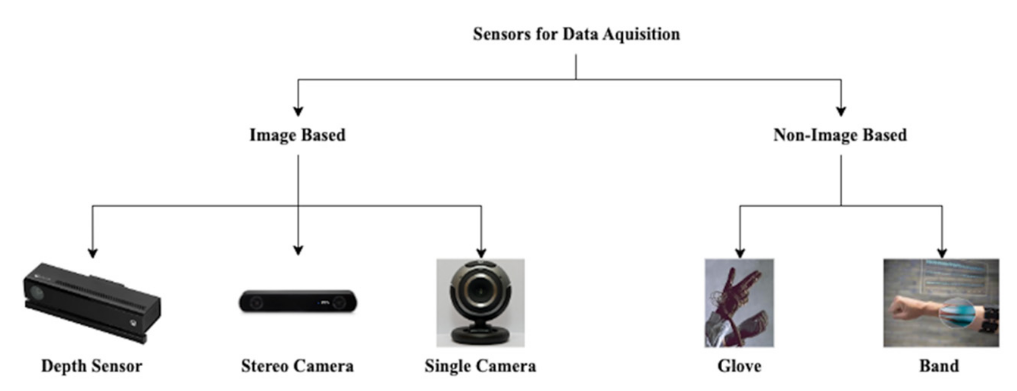
\includegraphics[scale=0.5]{figs/gesture_sensors.png}
    \caption{Flowchart showing the different types of gesture recognition approaches.}
    \label{fig:gesture_sensors}
\end{figure}

\subsection{Gesture Languages}
When a gesture is captured using either vision-based methods or non-vision based methods, movements of the hand are captured, however, theses movemnts need to be interpreted to give them meaning. For example, if a user moves their hand to the left, this movement needs to be interpreted as a command for the drone to move left. In order to do this, a gesture language is needed. Simply put, a gesture language is a dataset that matches a gesture to a specific meaning \citep{Patrona2021}. There are a numebr of different languages that have been used in the past for gesture recognition and have commonly been used to communicate between manned aerial vehicles. \cite{Patrona2021} expalins that aeroplane pilotes and helicopter pilots have been using hand gestures to communicate with each other for a number of years. 

These gestures have also been used to communicate with other unmanned vehicles, most notably drones. \cite{Patrona2021} lists the some of the most common gesture languages used to communicate with arial vehicles: 

\begin{itemize}
    \item \textbf{Naval Air Training and Operating Procedures Standardization (NATOPS).} This is the most complete and detailed dataset, used for communicating between a pilot of a aircraft or helicopter and the ground crew. This meanis that it cannot be used for drone control as "The way UAVs "perceive" what they see is totally different from the way humans do so." \citep{Patrona2021}.    
    \item \textbf{DJI Spark Language}. This lanugae was launched in 2017 as the first commerciral UAV to have gesture control for handeling the movement of the drone as well as image/video capturing. It consists of 8 gestures, namely: "palm launch, palm control, adjusting position, stop adjusting position, follow, take selfie, record video, beckon and palm land" 
    \item \textbf{DJI Mavic Air Lanhuage.} This language is similar to the DJI Spark language, however with a few alternations and additions to the gestures. 
    \item \textbf{Keck Gesture Dataset.} This is a subset of the NATOPS language and it consists of 14 gestures that were designd to be used in a cluttered environment with moving cameras. Its is primeraley used to validate other gesture languages as it is a framework with 126 videos of static gesrtures and 168 videos of gesutuses in a dynamic environment \citep{Esclara2017}. 
    \item \textbf{UAV-GESTURE Dataset.} This dataset was created in 2018 and was the first publically available dataset of "UAV handling signals recoprded outdoors by a flying drone." \citep{Patrona2021}. 
    \item \textbf{AUTH UAV Gesture LAnguage}. This dataset was created by \cite{Patrona2021} as a more generic language for controlling a dataset that improved on the limitations of the previously mentioned datasets. 
  
\end{itemize}
Although these gesture languages and datasets are effective for drone control, they are limited by the need for users to learn application-specific gestures. This restricts the ability to personalise the interaction, meaning users cannot easily employ natural gestures or tailor the system to suit their own requirements. The aim of this project is therefore to bridge this gap by allowing users to design and customise their own drone control gestures.

\section{Current Implementations}
There have been a numebr of implementations of gesture control for drones. They range in their application, harware implementations as well  as software implementations. A few will be discussed in this report 

\subsection{Wearable Glove Control}
One of the most comman implementations of gesture controlled drones has been to use a wearable device. The basic idea is that the drone mimics the movements of the hand and incorporates additional sensors to capture a wide range of gestures. A study by \cite{muezzinoglu2021} proposed an intelligent human-UAV interaction framework that was cenetered around the use of two wearable gloves that allowed for real-time, controller-free piloting of a drone. 

Each glove is made up of 5 flex sensors that are used to capture the bending movemnts of the fingers. These sensors are made of a resistive material that changes its resistance when bent. As the resistance changes an analog signal is created and can be processed to determine the shape of the hand. The gloves also make use of an IMU incorporating a 3-axis gyroscope and 3-axis accelerometer. These sensors work together to capture the orientation and movement of the hand. The data is then captured using an STM32 microcontroller. 

Figure \ref{fig:data_glove} depicts the design of the glove \citep{muezzinoglu2021}. 

\begin{figure} [htbp]
    \centering
    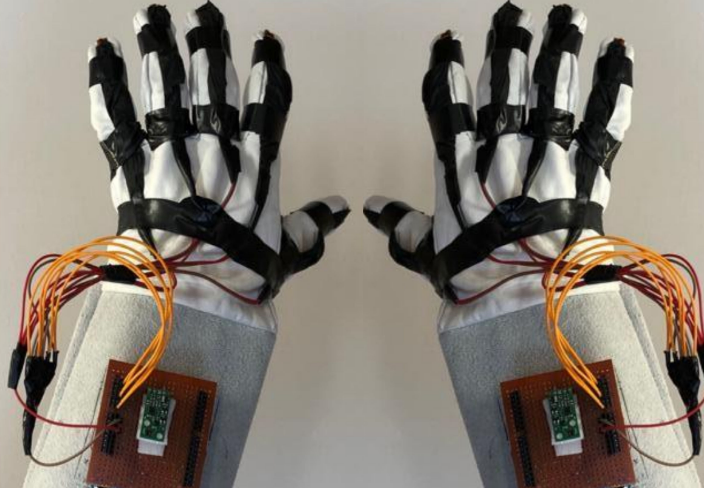
\includegraphics[scale=0.5]{figs/data_glove.png}
    \caption{Design of the wearable glove used for gesture control of a drone.}
    \label{fig:data_glove}
\end{figure}

As the user moves their hands and creates gestures, the sensors capture these signals. These signals are pre-processed by trimming and normalising the data. The signal triming phase is used to remove the first and last 3~\% of the signal data to eliminate any electrical noise as well as the noise created by transitioning between different gestures. The normalisation phase is used to normalise the raw analog-to-digital values into a consistent dataset to ensure that different users produce recognisable data patterns.  

Following this pre-processing, the framework employs a machine learning inference to classify the processed data into one of 25 distinct hand gestures.The researchers evaluated four specific machine learning algorithms to determine the most effective model for real-time flight control: Decision Tree (DT), Naive Bayes (NB), Support Vector Machine (SVM), and K-Nearest Neighbors (KNN). The experimental results revealed critical trade-offs between classification accuracy and computational speed. SVM was found to be the most precise model, achieving a mean accuracy of 98.02\%, though it required the longest training time at approximately 20~666.7 ms. For real-time piloting where low latency is paramount, KNN proved superior, delivering the fastest test time of 1.22 ms. Decision Tree offered the most efficient training phase at 133.1 ms, while maintaining a competitive accuracy of 96.96\%.

Once a gesture is recognized, the system utilizes a task scheduling algorithm to translate the identified class into pre-defined UAV flight commands. This multi-mode command structure allows for complex 3D navigation; for instance, specific hand orientations and finger flexions can trigger simultaneous movements such as ``Forward Up'' or ``Turn Left Down''. This glove-based approach offers a significant engineering advantage over vision-based systems, as it remains robust against variable ambient lighting and line-of-sight obstructions that typically hinder camera-reliant gesture recognition. The system's high accuracy and millisecond-level response times demonstrate its viability for high-precision human-UAV interaction in complex environments. One downside to this design is that it requires the user to wear a glove, making the device "intrusive and constraining for the user" \citep{Gio2021}. 

\subsection{Skywriter HAT sensor}
\cite{Mehta2023} made use of a near-field elctric field sensor (Skywriter HAT sensor shown in Figure \ref{fig:skywriter_hat} \citep{Skywriter_HAT}) to control the roll, pitch and yaw of a drone. The sensor detects a change in a magnetic field when a conducticve object (such as a hand) enters in the field. The change in magnetic field is converted into a digital signal that represents the x, y and z coordinate values. These values are used by a Raspberry Pi that converts these values into the roll, pitch and yaw control signals of a Crazyflie drone. An Extended Kalmen Filter was used to smooth the signals noise and to combine the information into one reliable estimate of the drone's position, velocity, and orientation at any moment.

\begin{figure} [htbp]
    \centering
    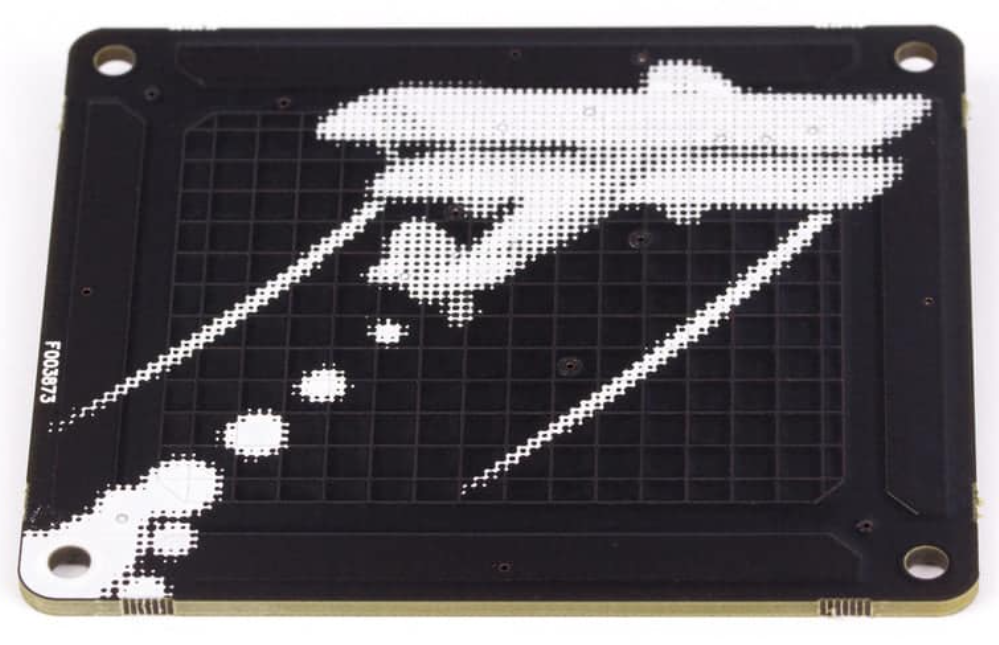
\includegraphics[scale=0.4]{figs/skywriter_hat.png}
    \caption{Skywriter HAT sensor used for gesture control of a drone.}
    \label{fig:skywriter_hat}
\end{figure}

The authors reported some success with this design; however, it also presented notable limitations and concerns. In particular, the Skywriter sensor was noisy, and the researchers were unable to fully isolate which axis was being moved. As a result, the drone drifted even when the user’s hand remained stationary.  

\subsection{LEAP Motion Sensor}
\cite{Sarkar2016} describes the Leap Montion Sensor as a gesture recognition device that uses two monochromatic infrared (IR) cameras and three infrared LEDs to track infrared light. By using stereoscopy from its two cameras, the Leap reduces errors and achieves highly precise tracking of hand and finger movements. The sensor can track hand motion up to a distance of about 1 meter directly above it, creating a hemispherical area above the sensor. Once the hand enters the area, the sensors detects movement and using the LEAP Software Development Kit (SDK), advanced Computer Vision algorithems run in order to exctract raw sensor data. Figure \ref{fig:Leap_sensor} \citep{Sarkar2016} shows the motion sensor as well as the area where a hand movement can be detected. 

\begin{figure} [htbp]
    \centering
    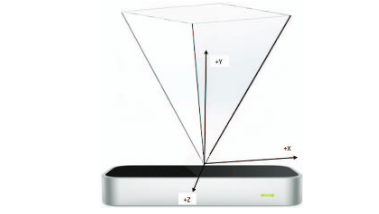
\includegraphics[scale=0.8]{figs/Leap_sensor.png}
    \caption{Leap motion sensor}
    \label{fig:Leap_sensor}
\end{figure}

The Leap motion sensor has been used by \cite{Sarkar2016} as a ground station to control the movements of an AR DRONE 2.0. However this sensor was only used to control the pitch, yaw and roll of the drone and it was not used to communicate any higher level commands to the drone.  

\subsection{Microsoft Kinect}
\cite{Gio2021} developed a system that uses the Microsoft Kinect to record full body gestures that were used to control a drone. The Microsoft Kinect is a depth-sensing device that captures the full body movements by constructing a real-time 3D skeletal model of a user. This model tracts the positions of the users jouints (eg. shoulders, elbows, spine and hips) which allows the system to track the posture and movement of a user. The gesture recognition is done by computing the angles between the joints rather than relying on the absolute positions of the body parts (e.g. arms, shoulders and hands). These calculated angles are compared to experimentally defined thresholds to determine which gesture is being peformed. This allows for gestures to be interperated, regardless of the users's body size or the distance from the sensor, making the system more felxible for users. Figure \ref{fig:Kinect_overview} shows a flow chart of how the system interacts with each subsystem \citep{Gio2021}.

\begin{figure} [htbp]
    \centering
    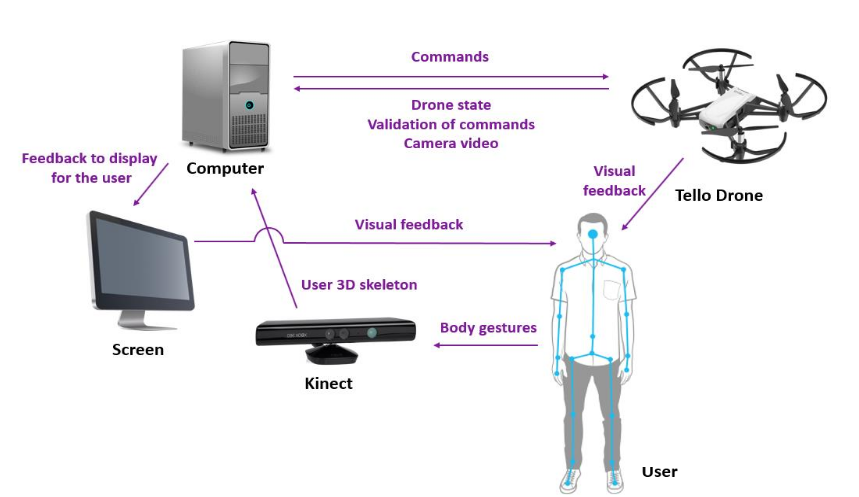
\includegraphics[scale=0.6]{figs/kinect_overview.png}
    \caption{Overview of the Microsoft Kinect system for drone control}
    \label{fig:Kinect_overview}
\end{figure}

The Kinect streams the joint position data to a computer, where the motion recognition software evaluates the geometroc relationships between the various joints. These relationships and angles correspond to drone commands such as move forward, sideways or rotate. Figure \ref{fig:Kinect_commands} shows the commands and the associated gestures that \cite{Gio2021} has developed.

\begin{figure} [htbp]
    \centering
    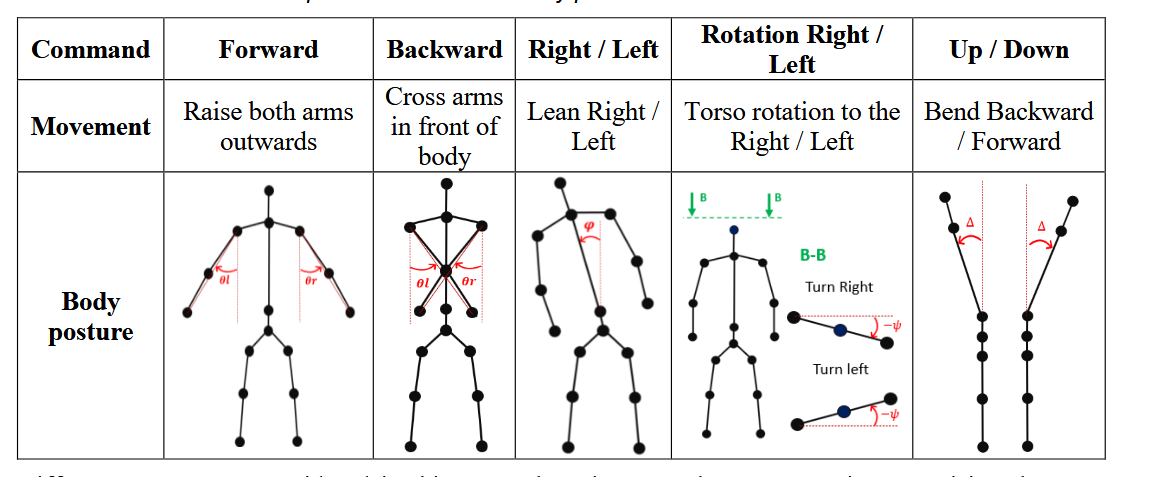
\includegraphics[scale=0.45]{figs/Kinect_gestures.png}
    \caption{Commands and associated gestures for the Microsoft Kinect system}
    \label{fig:Kinect_commands}
\end{figure}

One key contribution of this work is its implementation of speed control, which is achieved using the amplitude of the user's movements. Instead of gestures acting a simple on/off commands, the magnitude of the body motion is mapped to the drones velocity. Larger movements correspond to a higher speed command where as smaller, less pronounced movements result in lower speed commands. This form of control was achieved using a continuous linear mapping between the gesture amplitude and the speed of the gesture. Figure \ref{fig:Kinect_speed_control} \citep{Gio2021} shows how the amplitude and speed of the gestrure is used to control the speed of the drone.

\begin{figure}[htbp]
    \centering
    
    \begin{subfigure}[b]{0.45\textwidth}
        \centering
        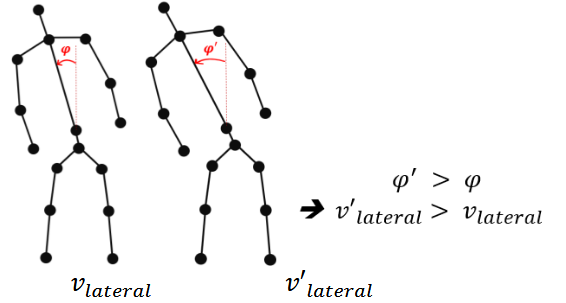
\includegraphics[scale=0.42]{figs/kinect_speed1.png}
        \caption{Diagram showing the control of the spped for a lateral movemnt of the drone.}
        \label{fig:image1}
    \end{subfigure}
    \hfill
    \begin{subfigure}[b]{0.45\textwidth}
        \centering
        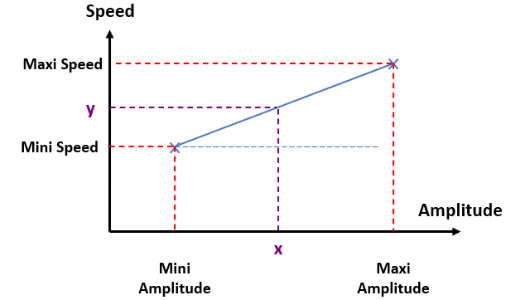
\includegraphics[scale=0.46]{figs/kinect_speed2.png}
        \caption{Graph showing the linear regression for speed calculation}
        \label{fig:image2}
    \end{subfigure}
    
    \caption{Speed control of the Kinect system}
    \label{fig:Kinect_speed_control}
\end{figure}

Figure \ref{fig:image1} shows that the angle $\varphi ' $ is greater than $\varphi$; which results in the lateral speed $v'_{lateral}$ of the drone being greater than the lateral speed $v_{lateral}$ of the drone. The following formulas are used to caluclate the gradient and the equation for the linear regression line shown in Figure \ref{fig:image2}:

\begin{equation}
    m = \frac{\text{maxi Speed} - \text{mini Speed}}{\text{maxi Amplitude} - \text{mini Amplitude}}
\end{equation}

\begin{equation}
    y = (x - \text{mini Amplitude}) \times m + \text{mini Speed}
\end{equation}

\cite{Gio2021} peformed a flight test to evaluate the systems peformance. The experiment was designed to reflect realistic future applications and required participants to navigate the drone to a target location while avoiding obstacles, capture an image, and return to the starting point. Both experienced and inexperienced users were included to represent professional and casual use cases. Although live video from the drone’s onboard camera was displayed, the test was carried out in an open space to ensure that less experienced users could still maintain direct visual contact with the drone. To enable comparison, the same task was performed using both gesture-based control and a traditional controller. Four participants took part: one experienced with both control methods, one familiar only with conventional control, and two with no prior drone experience. Users were given a brief explanation of the gestures and a 30-second practice period for each method, and each participant completed the task twice to ensure reliable data collection. The results are summarised in Figure \ref{fig:Kinect_results}.

\begin{figure} [htbp]
    \centering
    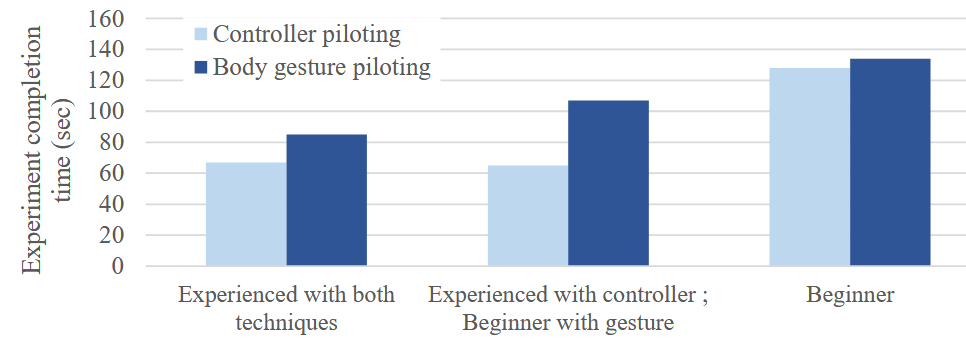
\includegraphics[scale=0.5]{figs/Kinect_results.png}
    \caption{Results of the Kinect gesture control experiment}
    \label{fig:Kinect_results}
\end{figure}

The results demonstrate that the Kinect-based gesture control system is both reliable and effective for drone operation. Gesture recognition was successful for all participants, regardless of physical differences, confirming the robustness of the angle-based tracking approach. The system also showed high accuracy, with less than 2~\% error between intended and executed speed commands, indicating precise translation of gestures into control actions. In practical flight tests, all users—including beginners, were able to complete navigation tasks successfully, although gesture-based control was about 27~\% slower for experienced users compared to a traditional controller. Despite this, the system was found to be more intuitive and less mentally demanding, particularly for inexperienced users, highlighting its potential as a natural and user-friendly alternative to conventional drone control.

\subsection{MediaPipe Hands}

A widely used image-based gesture control system in research is Google's MediaPipe Hands (MPH) framework. \cite{Khaksar2023} has used this software to develop a quadcopter control system as an alternative Human-Computer Inteaction (HCI) approach, focusing on replacing conventional drone control methods with a Hand-Gestuer Recognition (HGR) interface. The aim of this system was to develope and evaluate a HGR system capable of providing an intuative, low-cost, and reliable means of controlling a quatcopter without the neeed for specialised controllers or wearable hardware. 

The cental element of this system is the MPH framework. The authors descibe the MPH framework as an on-device real-time hand identification software, designed to operate using a single RGB camera. 
MPH operates using a two-stage machine-learning pipeline: first, a palm detection model identifies regions of interest within an RGB image, and second, a hand landmark model estimates a 21-point skeletal representation of the detected hand. Figure \ref{fig:MediaPipe_hand} shows the landmarks of the hand \citep{Taylor2025}.

\begin{figure} [htbp]
    \centering
    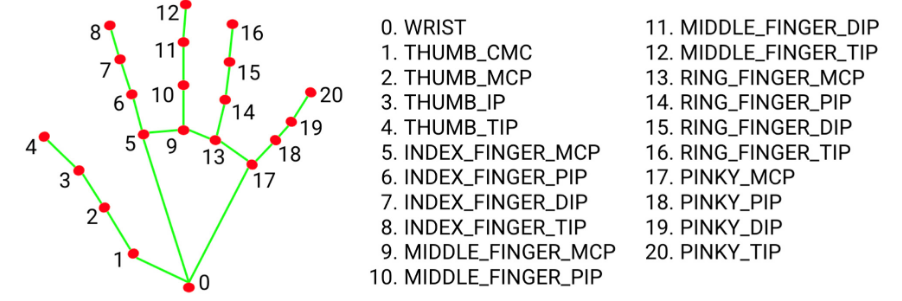
\includegraphics[scale=0.5]{figs/MediaPipe_hand.png}
    \caption{Landmarks identified by MediaPipe Hands}
    \label{fig:MediaPipe_hand}
\end{figure}

These landmarks provode a 2.5D representation (inferring depth) that allows for the calculation of joint angles and spatial relationships between the fingers. A quantitative validation was performed by comparing these computed joint angles with clinically measured values using a goniometer, allowing the authors to assess model accuracy under different hand poses and orientations. Finally, multiple classification algorithms are tested to determine the most accurate and efficient method for mapping gestures to predefined drone commands, and the system was implemented and tuned through real-world flight tests.

However, a limitation of MPH is that it is sensative to depth (Z-axis) variations \citep{Khaksar2023}, wich could reduce the landmark accuracy under certain conditions. It was found that the landmark accuaracy decreased from 86.7\% to 41.5\% under certain conditions. Despite these limitations, the system authors proposed a classification method that greatly improved the accuracy and allowed for the to maintain reliable performance achiving a gesture-calssification accuracy of 96.25\% in real-world flight tests.

Additionally, \cite{Taylor2025} has built on the use of MediaPipe Hands for gesture control of drones.  Making use of the 21 landmaks, the authors were able to implement a custom function that extracts two types of featires from the landmark data. These include: 

\begin{itemize}
    \item \textbf{Distance features}: 
    The eclidean distacne between specific landmarks were calculated as shown in Equation \ref{eq:Dist}. 
    \begin{equation}
        d_{ij} =  \left|{v_i - v_j} \right| = \sqrt{(x_i - x_j)^2 + (y_i - y_j)^2}
        \label{eq:Dist}
    \end{equation}
    
    \item \textbf{Angle features}:
    $\theta_{ijk}$ was defined using the cosine rule (Equation \ref{eq:arccos}) to measue the geometric angles between three consecutive landmarks, for example the finger joints. 
    \begin{equation}
        \theta_{ijk} = \arccos (\frac{(v_i - v_j)^T (v_k - v_j)}{d_{ij} \cdot d_{kj}})
        \label{eq:arccos}
    \end{equation}

\end{itemize}
 
Using these equations, a gesture matrix is constructed, mapping each equation output to a specific gesture command, as illustrated in Figure \ref{fig:Gesture_matrix} \citep{Taylor2025}.

 \begin{figure} [htbp]
    \raggedright
    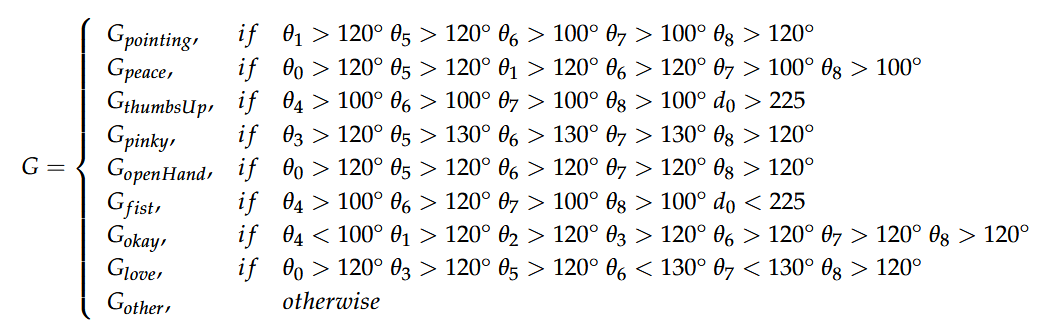
\includegraphics[scale=0.5]{figs/Gesture_matrix.png}
    \caption{Gesture matrix defining specific gestures based on distance and angle features extracted from the MediaPipe Hands landmarks.}
    \label{fig:Gesture_matrix}
\end{figure}

The results of this system showed that 8 of the 10 gestures reached a 100~\% recognition rate, however there were minor inconsistancies with the "peace" gesture achieving an accuracy of 88~\% and the "thumbs up" gesture achieving an accuracy of 96~\% as these appeared similar to other gestures. Thus the researchers concluded that the system successfully bridges the gap between human interaction and autonomous safety. While this system was shown to be effective, the researchers identified that the lighting conditions, hand positioning, and computational overhead were the primary areas for future optimization. 

\subsection{DJI Neo 2}
The most recent and advanced commercially available drone that uses gesture recognition to control its movement is the DJI Neo 2. This drone was released in November 2025 \citep{Kieldsen2025}. Due to this drone being very new there is little information available about the specific gesture recognition system that it uses, however the unique features of the drone are known. They include: 

\begin{itemize}
    \item Palm takeoff and landing 
    \item Distance control 
    \item Position Control
\end{itemize}

According to the user manual \citep{DJI_Neo2_Manual}, the drone can be controlled through the following gestures. When activated, the user must raise their palm towards the camera, the drone will then indicate with a blue light that the drone can be controlled with gestures. The drone then tracks the position of the user's hand and can move in the direction of the hand movement. For example, if the user moves their hand to the left, the drone will move to the left. If the user moves their hand up, the drone will move up. This is decsribed in Figure \ref{fig:DJI_Move}.

\begin{figure} [htbp]
    \centering
    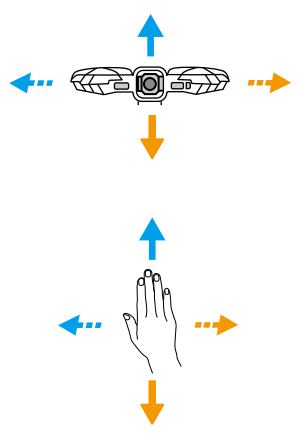
\includegraphics[scale=0.6]{figs/DJI_Move.png}
    \caption{Position control of the DJI Neo 2 using hand gestures.}
    \label{fig:DJI_Move}
\end{figure}

The drone can also be controlled by moving the hand closer or further away from the camera, which will control the distance of the drone from the user. This is done by moving both hands closer together to bring the drone closer, and moving them further apart to move it further away as seen in Figure \ref{fig:DJI_Dist} \citep{DJI_Neo2_Manual}.  

\begin{figure} [htbp]
    \centering
    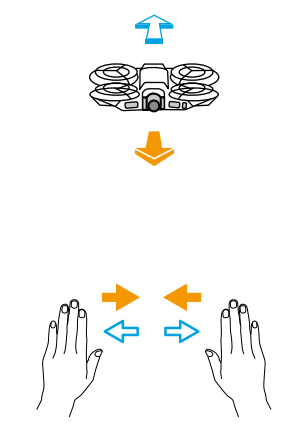
\includegraphics[scale=0.6]{figs/DJI_Dist.png}
    \caption{Distance control of the DJI Neo 2 using hand gestures.}
    \label{fig:DJI_Dist}
\end{figure}

The The drone has additional festures however that are not controlled with a gesture, but instead by using buttons on the drone itself. Some of these additonal features include ActiveTrack, Spotlight an Quickshots. The Quickshots feature on DJI drones are specific cinimatic shots that have a set flight path. These include: 

\begin{itemize}
    \item Dronie 
    \item Helix 
    \item Rocket 
    \item Circle 
    \item Boomearang
\end{itemize}

A notable limitation of this system is that gesture control is restricted to positioning the drone, with all additional functions requiring manual configuration on the drone itself or via a remote controller. This project therefore aims to address this limitation by developing a system capable of interpreting more complex gestural commands, enabling functions such as capturing photos, recording video, and activating specific flight modes to be done with a hand gesture. 

\subsection{EMG sensors}

\section{Gesture Classification Techniques}   
Having discussed the different types of gesture control and the current implementations of gesture control of drones, it is also important to discuss the different techniques that are used to recognise and classify gestures. There are a number of different techniques that have been used and the avancement of machine learnign has allowed for more accurate and efficient gesture recognition software. 

\subsection{Traditional Methods}
In this report, traditional methods refer to the well established and commonly used techniques used to recognise and classify gestures. Traditional hand gesture recognition (HGR) methods are based on a structured engineering approach that relies on manually designed features, rather than the automated feature learning used in modern deep learning systems \citep{jiashan2024}. These methods typically extract different types of features from the hand. Shape-based features are common and can include contour-based descriptors from specific regions, global region-based features such as Zernike moments, and gradient-based features like Histograms of Oriented Gradients (HOG), which capture local shape details \citep{bhushan2022}. For signal-based systems, such as those using wearable devices or infrared sensors, statistical measures are often used to describe the signal, including Variance (VAR), Root Mean Square (RMS), and Mean Absolute Value (MAV), which help quantify characteristics like amplitude and power. In addition, simple geometric properties—such as aspect ratio, subarea proportions, and the number of angular points—may be calculated to describe the hand's shape before classification \citep{nogales2023}.

Once these features are defined, they are passed to traditional classifiers. Common examples include K-Nearest Neighbors (KNN), which classifies data based on similarity to nearby samples using distance metrics, Support Vector Machines (SVM), which separate data using an optimal boundary or hyperplane, and Naive Bayes classifiers, which apply probability theory to determine the most likely class \citep{bhushan2022}. Decision Trees, which use measures like information gain and entropy to make decisions, are also widely used \citep{nogales2023}.

Despite their usefulness, these traditional methods have several limitations. Vision-based approaches are often sensitive to lighting conditions and obstructions, and for dynamic gestures, HMMs only consider transitions between consecutive states, which can overlook the overall coherence and structure of a gesture. DTW requires a predefined "standard" or reference gesture, which is often not available and must be set subjectively. Additionally, these systems can suffer from the "curse of dimensionality", where using too many features reduces performance and leads to overfitting, and they struggle to handle the natural variation in how different users perform the same gesture, both in space (spatial variability) and over time (variability of time) \citep{jiashan2024}. Some models, such as Naïve Bayes, rely on simplifying assumptions—like treating features as independent variables—which often fails to hold in practice and leads to unreliable results \citep{bhushan2022}.

More reliable and accurate approaches that are used are neural networks and deep learning algorithms to automate feature extraction \citep{jiashan2024}. 
Convolutional Neural Networks (CNNs), for instance, are highly effective at identifying unique grid patterns and extracting discriminative features directly from raw image data, bypassing the need for a manual detection or segmentation stage \citep{bhushan2022}. \cite{bhushan2022} demonstrated that CNNs significantly outperform traditional machine learning classifiers, achieving a peak accuracy of 91.41 \% on gesture datasets compared to much lower yields from models like Naïve Bayes or SVC. For dynamic gestures involving complex time sequences and spatial variability, advanced architectures such as 3D Convolutional Neural Networks (3DCNN) and Long Short-Term Memory (LSTM) networks are employed to capture temporal dependencies and ensure the continuity of the gesture motion \citep{jiashan2024}.  

However, although nearal networks have been shown to have superior accuracy, they present distinct engineering challenges. \cite{nogales2023} states that deep learning algorithms typically require high computational loads and significant programming complexity, which can hinder their portability. While the use of GPUs can mitigate processing delays, the high power consumption required by such hardware often conflicts with the requirements for portable, embedded hand gesture recognition systems. Furthermore, researchers have noted that it remains difficult to design neural network architectures that fully account for specific physical gesture motion features, sometimes leading to a "rough" treatment of time series data compared to more specialized geometric models \citep{jiashan2024}.  

\section{New Advancements}
There has been much development in the field of gesture control that goes beyond controlling drones. These developments have lead to new ways of interacting with robots and have also allowed for the development of new gesture recognition and classification techniques. The most relevent advancements are discussed below. 

\subsection{ToF Camera in Moving Vehicle}
\cite{Reyes2023} developed a system that uses a Time of Flight (ToF) camera to capture hand gestures in a moving vehicle. The aim f this research was to adress the challenges of dynamic hand gesture recognition within a driving environment. The researchers propose a model-adaptation approach to personalize a CNNLSTM (Convolutional Long-Short Term Memory) neural network, aiming to improve recognition accuracy while reducing the massive data requirements typically associated with deep learning. The system that was developed allowed a driver of a vehicle to control the infotainment system of the car using gestures to peform task such as increasing the volume, or skipping a song. It is important to note that the authors state that the system is designed to be expanded upon and adapted to be used in other applications. 

A ToF camera was chosen due to the limitations of RGB cameras in environments with variable lighting conditions. The data aquisition process involed the following: 
 \begin{itemize}
    \item \textbf{Camera setup}. The camera was mounted on the ceilign of the vehicel near the front of the car. This provided a top-down perspective of the gear shift area. 
    \item \textbf{Data collection}. 83 participants were asked to perform a series of six specified gestures. These gestures can be seen in Figure ** \citep{Reyes2023}. As a result the final dataset comprised of 4325 gestures. 
 \end{itemize} 

\begin{figure}[htbp]
    \centering
    
    \begin{subfigure}{0.2\textwidth}
        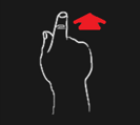
\includegraphics[width=\linewidth]{figs/point_tof.png}
    \end{subfigure}
    \begin{subfigure}{0.2\textwidth}
        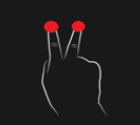
\includegraphics[width=\linewidth]{figs/2_finger_tof.png}
    \end{subfigure}
    \begin{subfigure}{0.2\textwidth}
        
\includegraphics[width=\linewidth]{figs/right_rotate_tof.png}
    \end{subfigure}    
    \begin{subfigure}{0.2\textwidth}
        
\includegraphics[width=\linewidth]{figs/left_rotate_tof.png}
    \end{subfigure}

    \vspace{0.5cm}

    \begin{subfigure}{0.2\textwidth}
        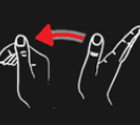
\includegraphics[width=\linewidth]{figs/swipe_left_tof.png}
    \end{subfigure}
    \begin{subfigure}{0.2\textwidth}
        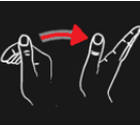
\includegraphics[width=\linewidth]{figs/swipe_right_tof.png}
    \end{subfigure}
    
    \caption{Six gestures performed by participants}
\end{figure}

The dataset then underwent a preprocessingng phase which included stadarising the data suc that eaahc recorded gesture was fiixed to 12 fps (frames per second), having a maximum of 70 frames s per gesture. Secondly a 3D region of interest was established to be within 12 - 500 cm from the camera to limit where a gestre could be peformed. Finally background subtraction was used to isolate the hand from background of the car. With this completed the data was then used to train a CNNLSTM model. 

The study highlight that a "one-model-fits-all" approach is insufficient due to individual differences in gesture performance. The model personalization and adaptation process begins with the creation of a Universal Background Model (UBM), a baseline CNNLSTM architecture trained on a broad group of participants that initially achieves a recognition accuracy of 66.9~\%. To account for the individual differences in how various users perform dynamic gestures, the researchers utilize fine-tuning to adapt this UBM to specific individuals within an "Adaptation Set". This single-step adaptation involves training the UBM for an additional 20 epochs using a small amount of data from the specific user, which increases recognition accuracy to 77.8~\%. The effectiveness of this personalization is further enhanced through data augmentation—using random translations along the X and Y axes to artificially expand the training set—which pushes the average personalized accuracy to 86.4~\%. Experimental results indicate that while the model improves with as few as two gestures per class, accuracy peaks at 90.5~\% when the model is fine-tuned with 20 gestures per class. Finally, the study explores incremental learning, where the vehicle adapts to the driver over time; however, this results in a "stability-plasticity dilemma" where the system becomes highly accurate for the specific user but "forgets" how to recognize gestures from others, a common side effect of deep learning personalization.

\subsection{One-shot Gesture Recognition}
\cite{Cabrera2017} identified a core problem with gesture recognition systems that being they require many training examples to work. As a result they developed a system that learns to recognise a gesture from a single observation. This is known as one-shot learning. Rather than collecting lots of training data and treating the data as purely statistical patterns, this framework extracts key "inflection points" from a single gesture and uses them to artificially generate hundreds of realistic variations that  are used for training \citep{Cabrera2017}. 

The inflection points that the authers use are not arbitary, but are instead neurologically motivated, correlating with electroencephalographic (EEG) signals in the motor cotex, reflecting the way humans naturally represent gestures in the brain.

The approach was evaluated using eight upper-limb gestures from the MSRC-12 Kinect dataset, across multiple classification techniques, including Dynamic Time Warping (DTW), Support Vector Machines (SVM), Hidden Markov Models (HMM), and Conditional Random Fields (CRF). Results demonstrated strong performance, achieving an average classification accuracy of approximately 90~\% across all classifiers. In addition to conventional accuracy metrics, the authors introduced a novel “coherency” measure, which evaluates the agreement between human and machine interpretation of gestures. Using a Baxter robot to perform the generated gestures, a coherency score of 93.8~\% was achieved, indicating a high level of alignment between artificial and human gesture recognition.

Furthermore, the system exhibits adaptive learning capabilities, where performance improves as additional real-world observations are incorporated. Accuracy was shown to increase from approximately 90~\% in the one-shot case to around 95~\% with ten training examples, illustrating a natural progression from one-shot to N-shot learning. However, a temporary decrease in performance at low sample sizes highlights the sensitivity of the system to outlier observations. This can be seen in Figure \ref{fig:AL_results} which shows the Adative Learning (AL) system implemented with two differrent classification algorithems: DTW and HMM. 

\begin{figure} [htbp]
    \centering
    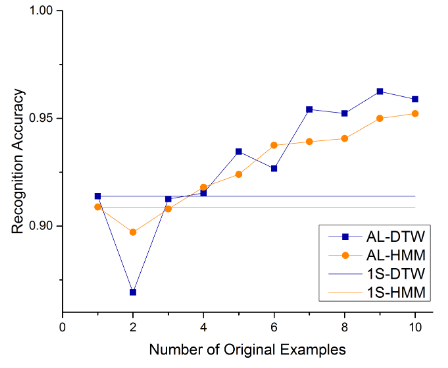
\includegraphics[scale=0.7]{figs/AL_results.png}
    \caption{Adaptive learning performance of the one-shot gesture recognition system, showing classification accuracy as a function of the number of training examples for both DTW and HMM classifiers.}
    \label{fig:AL_results}
\end{figure}

Overall, the key contribution of this work lies in its classifier-agnostic framework, which integrates principles from cognitive science with machine learning to enable robust recognition of previously unseen gestures from minimal training data.

\subsection{Vision-based hand gesture (FSL)}
Following on from this research \cite{Shahi2024} developed a system that also learns to recognise a gesture from a single observation. The authros of this research present a vision-based hand gesture recognition system that enables gesture customization from a single demonstaration. the system proposed by \cite{Shahi2024} devel;oped a end-to-end framework tha supports a wide range of gestures, including both static and dynamic, one and two-handed gestures as well as multiple viewpoints. The method combines hand keypoint extraction, a graph transformer architecture, and a few-shot learning (FSL) stratagy besed on meta-learning (MAML) to rapidly adapt to new gesture classes from minimal data. Hand pose estimation is used to extract skeletal joint coordinates, which are processed by the graph transformer to capture both the spatial relatiobships between the joints and the temporal motion patterns. To further enhance learning from limited data, a meta-augmnetation technique is introduced to increase task diversity by generating additional gesture combinations. Unlike many prior works, the system also incorporates a background calss to distinguish intential gestures from irrelevant hand movements, improving real world robustness. Figure \ref{fig:FSL_overview} discribes the system overview \citep{Shahi2024}. 

\begin{figure} [htbp]
    \centering
    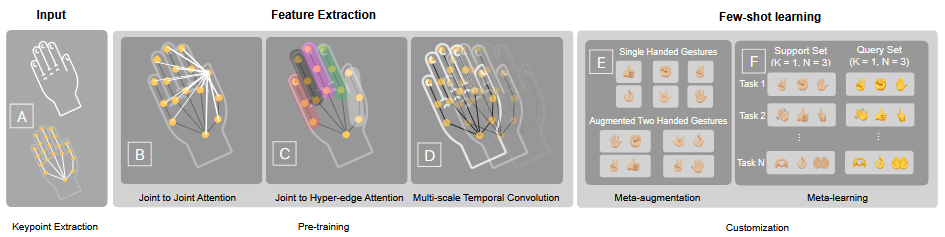
\includegraphics[scale=0.55]{figs/FSL_overview.png}
    \caption{Overview of the vision-based few-shot hand gesture recognition system.}
    \label{fig:FSL_overview}
\end{figure}

\cite{Shahi2024} evaluated the  system through a user study involving 21 participants and 20 gesture classes. The results show a average accuracy of 95~\% with only one demonstration per gesture. This show that the system outperforms baseline approaches such as fine-tuning, nearest neighbours and random forest classifiers. Additionally, the authors demonstrate the practicallity of their approach via theree real-wolrd applications, including a gesture design tool, gesture-based productivity interfaces, and mixed reality interaction systems.  


\chapter{Workplan}
This section outlines the proposed work plan for the project, detailing the key phases and activities required to achieve the stated objectives. The plan follows a structured approach, progressing from foundational research through system design, prototype development, testing, and final documentation.

\begin{itemize}

\item \textbf{Research} \\
A literature review will be conducted to develop an understanding of gesture control, its underlying principles, and its various applications. This review will help clarify the problem space, enabling a well-defined problem statement. It will also provide a basis for comparing existing gesture recognition techniques and implementations.

\item \textbf{Concept Definition}
\begin{itemize}
    \item \textbf{Aim and Objectives} \\
    This section will clearly define the overall aim of the project, along with the specific objectives required to achieve it.

    \item \textbf{Stakeholders’ Requirements} \\
    This will identify the needs and expectations of the end users. It will define who the system is intended for and outline the key functionalities and performance expectations from a user perspective.

    \item \textbf{Engineering Requirements} \\
    The technical requirements of the system will be established here, guided by the stakeholders’ needs. These requirements will translate user expectations into measurable engineering specifications.

    \item \textbf{Drone Selection} \\
    A comparison of potential drones will be conducted, highlighting the advantages and limitations of each option. This will support the selection of the most suitable platform for the project.
\end{itemize}

\item \textbf{System Architecture Design}
\begin{itemize}
    \item \textbf{Model Selection} \\
    A suitable gesture recognition and classification approach will be selected. This includes evaluating existing methods and identifying opportunities for improvement.

    \item \textbf{Model Development} \\
    The chosen model will be developed, including training procedures and parameter tuning.

    \item \textbf{Model Optimisation} \\
    The model will be refined to improve performance, accuracy, and computational efficiency.
\end{itemize}

\item \textbf{Prototype}
\begin{itemize}
    \item \textbf{Hardware Selection} \\
    Appropriate hardware components, such as cameras and sensors, will be selected. The drone selection is treated separately, as it significantly influences other hardware choices.

    \item \textbf{Assembly} \\
    The system components will be assembled into a functional prototype, including the final test drone setup.

    \item \textbf{Hardware Testing} \\
    The hardware will be tested to ensure reliable operation and to identify and resolve any faults.

    \item \textbf{Data Collection Protocol} \\
    A structured method will be designed for safely collecting and storing data from both the drone and the gesture recognition system.

    \item \textbf{Software Implementation} \\
    Once the hardware is operational and data collection methods are in place, the software will be integrated with the hardware, and initial system testing will begin.

    \item \textbf{Software Evaluation} \\
    System performance will be evaluated, and improvements will be made based on the results.

    \item \textbf{System Implementation} \\
    The fully integrated system will be tested in various environments and across different use-case scenarios to assess robustness and adaptability.

    \item \textbf{Ethics Approval} \\
    Ethical approval will be obtained, as the system testing involves human participants.

    \item \textbf{User Testing} \\
    Participants will be asked to perform a range of gestures to evaluate how effectively the system responds to different users and gesture variations.

    \item \textbf{Results Analysis} \\
    The collected data will be analysed to assess system performance and identify areas for improvement.
\end{itemize}

\item \textbf{Documentation} \\
The project report will be continuously developed throughout the project. This ensures that all findings, results, and insights are accurately recorded and preserved.

\end{itemize}

\chapter{Project Schedule}

This section provides an overview of the planned activities and timeline for the project.

\begin{landscape}

\begin{figure}
\centering\resizebox{\linewidth}{!}{
\begin{ganttchart}[
    hgrid,
    vgrid,
    x unit=0.5cm,
    y unit chart=0.9cm,
    bar label node/.append style={
        text width=3.7cm,
        align=left,
        font=\small\linespread{0.6}\selectfont
    },
    group label node/.append style={
        text width=3.7cm,
        align=left,
        font=\bfseries\linespread{0.6}\selectfont
    },
    milestone label node/.append style={
        text width=3.7cm,
        align=left,
    }
]{1}{50}

% ---- Months ----
\gantttitle{2026}{50} \\

\gantttitle{Jan}{3}
\gantttitle{Feb}{4}
\gantttitle{Mar}{4}
\gantttitle{Apr}{4}
\gantttitle{May}{5}
\gantttitle{Jun}{4}
\gantttitle{Jul}{5}
\gantttitle{Aug}{4}
\gantttitle{Sep}{4}
\gantttitle{Oct}{5}
\gantttitle{Nov}{4}
\gantttitle{Dec}{4} \\

% ---- Week numbers ----
\gantttitlelist
{16,23,30,
 6,13,20,27,
 6,13,20,27,
 3,10,17,24,
 1,8,15,22,29,
 5,12,19,26,
 3,10,17,24,31,
 7,14,21,28,
 4,11,18,25,
 2,9,16,23,30,
 6,13,20,27,
 4,11,18,25}{1} \\

% ---- Task bars ----
\ganttgroup{3.1 Research}{2}{23} \\
\ganttbar{3.1.1 Literature Review}{2}{23} \\
\ganttbar{3.1.2 Comparison of current implementations}{6}{14} \\
\ganttmilestone[name=MS1]{Project proposal (15 May)}{17} \\

\ganttgroup{3.2 Concept Definition}{9}{25} \\
\ganttbar{3.2.1 Aim and Objectives}{9}{11} \\
\ganttbar{3.2.2 Stakeholder requirements}{12}{14} \\
\ganttbar{3.2.3 Engineering Requirements}{15}{17} \\
\ganttbar{3.2.4 Drone Selection}{16}{20} \\
\ganttbar{3.2.5 Software selection}{21}{25} \\

\ganttgroup{3.3 System Architecture Design}{26}{48} \\
\ganttbar{3.3.1 Model Selection}{26}{36} \\
\ganttbar{3.3.2 Model Development}{29}{41} \\
\ganttbar{3.3.3 Model Optimisation}{42}{48} \\

\ganttgroup{3.4 Prototype }{32}{49} \\
\ganttbar{3.4.1 Hardware Selection}{32}{35} \\
\ganttbar{3.4.2 Assembly}{35}{39} \\
\ganttbar{3.4.3 Hardware testing}{38}{41} \\
\ganttbar{3.4.4 Data Collection Protocol}{42}{43} \\
\ganttbar{3.4.5 Software Implementation}{44}{49} \\

\ganttbar{\textbf{3.4 Documentation}}{4}{49}

\ganttlink[link mid=0.75]{elem5}{elem6}
\ganttlink{elem6}{elem7}
\ganttlink{elem8}{elem9}
\ganttlink{elem9}{elem11}
\ganttlink{elem12}{elem13}
\ganttlink{elem17}{elem18}
\ganttlink{elem18}{elem19}

\end{ganttchart}}
\caption{Gantt Chart 2026}
\label{fig:gantt2026}
\end{figure}

\begin{figure}
\centering\resizebox{\linewidth}{!}{
\begin{ganttchart}[
    hgrid,
    vgrid,
    x unit=0.5cm,
    y unit chart=0.9cm,
    bar label node/.append style={
        text width=3.7cm,
        align=left,
        font=\small\linespread{0.6}\selectfont
    },
    group label node/.append style={
        text width=3.7cm,
        align=left,
        font=\bfseries\linespread{0.6}\selectfont
    },
    milestone label node/.append style={
        text width=3.7cm,
        align=left,
    }
]{1}{39}

% ---- Months ----
\gantttitle{2027}{39} \\

\gantttitle{Jan}{5}
\gantttitle{Feb}{4}
\gantttitle{Mar}{4}
\gantttitle{Apr}{5}
\gantttitle{May}{4}
\gantttitle{Jun}{4}
\gantttitle{Jul}{5}
\gantttitle{Aug}{4}
\gantttitle{Sep}{4} \\

% ---- Week numbers ----
\gantttitlelist
{1,8,15,22,29,
 5,12,19,26,
 5,12,19,26,
 2,9,16,23,30,
 7,14,21,28,
 4,11,18,25,
 2,9,16,23,30,
 6,13,20,27,
 3,10,17,24}{1} \\

% ---- Task bars ----
\ganttgroup{3.4 Prototype }{1}{31} \\
\ganttbar{3.4.5 Software Implementation}{1}{1} \\
\ganttbar{3.4.6 Software evaluation}{2}{6} \\
\ganttbar{System implementation}{7}{16} \\ 
\ganttbar{Ethics approval }{17}{20} \\ 
\ganttbar{User testing}{21}{24} \\
\ganttbar{Result analysis}{24}{34} \\


\ganttbar[name=documentation]{\textbf{3.4 Documentation}}{1}{37} \\

\ganttmilestone[name=MS2]{Thesis hand-in (10 Sep)}{37}

\ganttlink{elem1}{elem2}
\ganttlink{elem2}{elem3}
\ganttlink{elem3}{elem4}
\ganttlink{elem4}{elem5}
\ganttlink[link type=f-m]{documentation}{MS2}

\end{ganttchart}}
\caption{Gantt Chart 2027}
\label{fig:gantt2027}
\end{figure}

\end{landscape}
\chapter{Risk Assessment}
\noindent This section presents a risk assessment for the development, assembly, and testing of the gesture-controlled drone system. Potential hazards associated with each activity are identified and classified according to their impact on personal safety (P), equipment (E), or both. Appropriate mitigation strategies are proposed to reduce the likelihood and severity of each risk. The assessment follows a proactive approach, ensuring that safety, regulatory compliance, and system reliability are considered throughout all stages of the project.

{
\footnotesize
\setlength{\tabcolsep}{3pt}
\begin{longtable}{|>{\raggedright\arraybackslash}p{0.17\textwidth}|>{\raggedright\arraybackslash}p{0.25\textwidth}|>{\centering\arraybackslash}p{1.2cm}|>{\raggedright\arraybackslash}p{0.25\textwidth}|>{\centering\arraybackslash}p{2.0cm}|}
\caption{Risk assessment for gesture-controlled drone system.} \\
\hline
\rowcolor{gray!30}
\textbf{Activity} & \textbf{Risk} & \textbf{Risk Type* (P/E)} & \textbf{Mitigation} & \textbf{Risk Severity} \\
\hline
\endfirsthead

\hline
\rowcolor{gray!30}
\textbf{Activity} & \textbf{Risk} & \textbf{Risk Type* (P/E)} & \textbf{Mitigation} & \textbf{Risk Severity} \\
\hline
\endhead

\hline \multicolumn{5}{r}{\textit{Continued on next page}} \\
\endfoot
\hline
\endlastfoot

% ---------------- GENERAL ----------------
\multicolumn{5}{|l|}{\textbf{General}} \\
\hline
Ethics approval & Delay in approval prevents user testing & E & Submit ethics application early, ideally during concept phase & High \\
\hline
Flight operations & Flying without permits and breaches of regulations & P \& E & Identify regulations and obtain permits before flight & High \\
\hline
Hardware procurement & Delays in components delay entire project & E & Order early and identify backup suppliers. Additionally, purchase spare parts to account for faulty or damaged components & High \\
\hline
Battery storage & Fire risk from incorrect LiPo storage & P \& E & Store in LiPo bag and use approved chargers. Have an appropriate fire extinguisher near in the labs where the batteries are stored & High \\
\hline

% ---------------- SOFTWARE ----------------
\multicolumn{5}{|l|}{\textbf{Software}} \\
\hline
Gesture control & Misclassification causes unintended motion & P \& E & Implement kill switch and test in simulation first & High \\
\hline
Model optimisation & Excessive tuning delays project & E & Define stopping criteria and time-box optimisation & Medium \\
\hline
Data collection & Data loss or corruption during testing & E & Backup data regularly and save to multiple devices & Medium \\
\hline

% ---------------- ASSEMBLY ----------------
\multicolumn{5}{|l|}{\textbf{Assembly}} \\
\hline
Soldering & Burns or inhalation of fumes & P & Work in ventilated area and use proper handling & Low \\
\hline
Electronics handling & Damage from electrostatic discharge or overcharge & E & Ensure all components are grounded properly and power components at rated voltage and current settings & Low \\
\hline
Electrical connections & Shock from live wiring & P & Disconnect power before modifications & Medium \\
\hline
Battery handling & Fire from damaged LiPo battery & P \& E & Inspect batteries and avoid short circuits. Have quick access to appropriate fire extinguisher & High \\
\hline
Drone assembly & Cuts from sharp edges & P & Where appropriate personal protective equipment and sand sharp edges & Low \\
\hline
Tool use & Injury from slipping tools & P & Use correct tools and secure workpiece. Get appropriate training if needed & Low \\
\hline
Workbench & Accidents due to clutter & P \& E & Maintain clean and organised workspace & Low \\
\hline

% ---------------- TESTING ----------------
\multicolumn{5}{|l|}{\textbf{Testing}} \\
\hline
Initial flight tests & Collision with people or objects & P \& E & Use safety zone, prop guards, and spotter & High \\
\hline
User testing & Injury due to incorrect gesture response & P \& E & Maintain safe distance and manual override & High \\
\hline
Outdoor testing & Loss of control (flyaway) & P \& E & Use RC override and test in enclosed areas & High \\
\hline
Environmental conditions & Wind or obstacles cause collision & P & Take precautions to plan tests to mitigate environmental interference. & Medium \\
\hline
Pre-flight checks & Battery failure causes crash & P & Inspect and monitor batteries before flight & High \\
\hline
Hardware failure & Loss of vision/processing mid-flight & P \& E & Implement watchdog and pre-flight checks & Medium \\
\hline

\end{longtable}

\par\medskip\noindent\textit{*P -- Personal, E -- Equipment}
}

%\include{chaps-main/chap-content-A}
%\include{chaps-main/chap-conclusion}

\appendix%------------------------------------------------------------
%\include{chaps-append/chap-maths}
%\include{chaps-append/chap-experiment}

\backmatter%----------------------------------------------------------
\bibliography{bib/bib-reference.bib}
 
\end{document}   

